\documentclass[11pt]{hw-template}

\usepackage{enumitem}
\usepackage{graphicx}
%\usepackage{mathtools}
%\lstset{showstringspaces=false}
%\setlength\parindent{0pt}

\coursename{Continuous Buhmbox Formulation} % DON'T CHANGE THIS

\studname{Alexandre Lamy}
\studmail{all2187@columbia.edu}
\hwNo{}
\collab{}

\begin{document}
\maketitle

\section*{Buhmbox generalization to continuous phenotypes - no cases and controls}

\noindent Assuming normalized weights ($\sum \omega_i = 1$), we define the weighted mean as:
$$m(x, \omega) = \sum_i \omega_i x_i$$
The weighted covariance as:
$$cov(x, y, \omega) = \sum_i \omega_i(x_i - m(x, \omega))(y_i - m(y, \omega))$$
Finally we have that the weighted correlation is given by:
$$corr(x, y, \omega) = \frac{cov(x, y, \omega)}{\sqrt{cov(x, x, \omega)cov(y, y, \omega)}}$$

Assume we are given $N$ data points (each data point corresponds to an individual's SNPs, $x_i \in \R$, and his phenotype, $y_i \in \R$). We have to further assume that the sample is 
representative of the population.

We then use $\omega_i = -log(1-\rho_i)$ where $\rho_i$ is the percentile of data point $x_i's$ phenotype (and then normalize the $w_i$'s to have $\sum w_i = 1$). We also let $R$ be the weighted
covariance matrix and $R'$ be the unweighted covariance matrix.
Then we use:
$$ Y = \frac{1}{\sqrt{\frac{1}{N} + \sum \omega_i^2}} (R-R')$$

$$S_\text{BUHMBOX} = \frac{\sum_{i < j} w_{ij}y_{ij}}{\sqrt{\sum_{i<j}w_{ij}^2}}$$

Where we have
$$w_{ij} = \frac{\sqrt{p_i(1-p_i)p_j(1-p_j)}(\gamma_i - 1)(\gamma_j - 1)}{((\gamma_i-1)p_i + 1)((\gamma_j - 1)p_j + 1)}$$

Where $p_i$ is the RAF of SNP $i$ and $\gamma_i$ is given by:
$\gamma_i = \frac{(p_i^+)(1-p_i^+)}{(p_i^-)(1-p_i^-)}$ where $p_i^+$ is the weighted sample RAF (using $\omega$ weights) and $p_i^-$ is the unweighted sample RAF.
%%%%%%%%%%%%%%%%%

\section*{Results}

As on 10/16 used three sets of data: independent, pleiotropic, heterogeneous. Each population is generated with 100000 individuals. Results after 100 runs (over 2 hrs).
\begin{table}[h!]
    \begin{tabular}{lll}
      \textbf{Population} & \textbf{BB with threshold - mean, sd} & \textbf{Continuous BB - mean, sd} \\
      Independent   & 0.14, 1.00     &  0.27, 0.68 \\
      Pleiotropic   & -12.60, 0.75   &  -17.52, 0.86\\
      Heterogeneous & 29.10, 1.10    &  34.62, 0.99
    \end{tabular}
\end{table}

The threshold used in the first case was z=1.5 (about 7000 cases). No noise was added when doing data generation. So heritability is 1.

\Oldsection*{Tasks}
\begin{itemize}
  \item Vectorize BB code and data generation (expected speedup of $\approx 100x$)
  \item Add noise and test with low heritabilities.
  \item Try different weight functions.
\end{itemize}

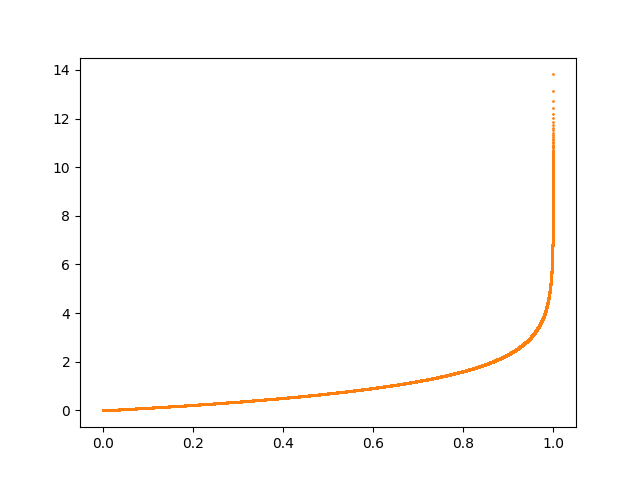
\includegraphics[width=0.99\linewidth]{log.png}

\end{document} 
